\documentclass{article}

% Paquetes
\usepackage[utf8]{inputenc}
\usepackage[T1]{fontenc}
\usepackage[spanish, mexico]{babel}
\usepackage{fullpage}
\usepackage{setspace}
\onehalfspacing
\usepackage{graphicx}

\usepackage{amsfonts}
\usepackage{amsmath}
\usepackage{amsthm}

% Mis definiciones
%% Teoremas 
\newtheorem{lema}{Lema}

%% Comandos
\newcommand{\RR}{\mathbb{R}}
\newcommand{\dd}[1]{\textrm{d}#1}

%% Operadores
\DeclareMathOperator{\signo}{sign}

\title{El algoritmo perceptron en 2--dimensiones}
\author{Juan M Barrios}
\date{\today}

\begin{document}

\maketitle

\section{Introduction}

El algoritmo del \textbf{perceptrón} resuelve un problema de clasificación binaria siempre que las observaciones
se puedan separar de manera lineal, esto lo hace encontrando un \emph{hiperplano} el cual sirve como frontera 
entre los dos comportamientos de los datos. Este algortimo fue publicado en 1958 por Frank Rosenblatt.

\begin{figure}
    \centering
    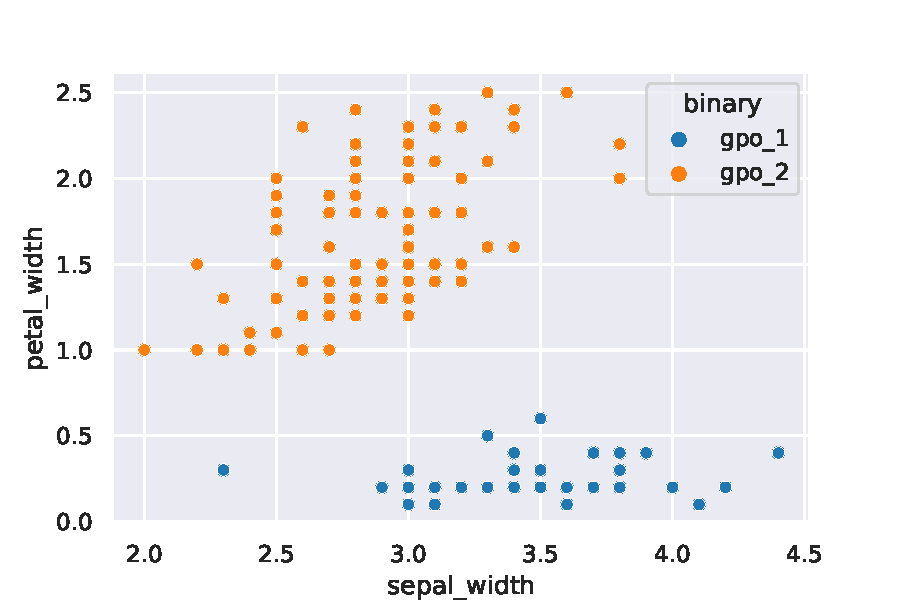
\includegraphics[width=.5\textwidth]{./imgs/plotdata}
    \caption{Ejemplo de datos linealmente separables}
    \label{fig:plotdata}
\end{figure}

\section{Ecuación de una recta y el producto punto}
Supongamos que tenemos dos vectores $\vec{u}, \vec{v}$ en $\RR^2$ se define el \emph{producto punto} (o producto 
escalar) como
$$
\vec{u}\cdot\vec{v} = (u_1, u_2)\cdot(v_1, v_2) = u_1v_1 + u_2v_2. \int_a^bf(x)\dd{x}
$$

Con esto podemos escribir una recta en $\RR^2$ como 
\begin{equation}\label{e:rectaparametrica}
    \vec{u}\cdot\vec{x} + \gamma = 0,
\end{equation}
está ecuación se le conoce como \emph{representación paramétrica} de la rectala y la cual no es la 
ecuación de la recta que conocimos en la preparatoria la cual era $y=mx+b$, donde $m$ era la  pendiente 
y $b$ la coordenada al origen.

\begin{lema}
La ecuación~\ref{e:rectaparametrica} cumple la ecuación normal de la recta.
\end{lema}
\begin{proof}
Sea $\vec{x} = (x, y)$ y $\vec{u}=(u_1, u_2)$ entonces 
\begin{align*}
    \vec{u}\cdot\vec{x} + \gamma &= u_1x + u_2y + \gamma\\
                        &= u_2(\frac{u_1}{u_2}x + y + \frac{\gamma}{u_2})
\end{align*}
entonces de~\eqref{e:rectaparametrica} se sigue que 
$$
    y = -\frac{u_1}{u_2}x - \gamma/u_2
$$
por lo que $m=-\frac{u_1}{u_2}$ y $b=-\frac{\gamma}{u_2}$
\end{proof}


Lo van a ocupar
$$
    \signo(x) = \begin{cases}
                    \phantom{-}1 & \textrm{si } x \textrm{ es no negativo} \\
                    -1 & \textrm{si } x \textrm{ es negativo}
               \end{cases}
$$
\end{document}
